
\documentclass[11pt,a4paper]{article}
\usepackage[left=2cm,right=2cm,top=2cm,bottom=3cm]{geometry}
\usepackage{amsmath,amsfonts,amsthm,amssymb,varioref,times, commath}
\usepackage{gensymb}
\usepackage{tikz}
\usepackage{textcomp}
\usepackage{hyperref}
\hypersetup{
 colorlinks=true,
 linkcolor=blue,
 filecolor=magenta, 
urlcolor=cyan,
}
\usepackage{lipsum}
\usepackage{epigraph}
%to resume numbering in a list
\usepackage{enumitem}
%----- arrows 
\usepackage{extarrows}

%    differential equatiosn 
\usepackage{diffcoeff}   %\diff[2]{x}{y}


%%%%%%pour ecrire en français avec les accents
\usepackage[utf8]{inputenc}
\usepackage[T1]{fontenc}
\usepackage{lmodern} % load a font with all the characters
\usepackage{units}
%%%%%%%Image-related packages
\usepackage{wrapfig}
\usepackage{float, graphicx}
\graphicspath{ {./img/} }
\usepackage{subcaption}
\usepackage[export]{adjustbox}

%%%%%%%pour faire des cadres
\usepackage{xcolor}
\usepackage{tcolorbox}
\usepackage{framed}
\usepackage{mdframed}


%%%%%%%chemistry frmulae
\usepackage{chemfig}
\usepackage{chemformula}
\usepackage[version=4]{mhchem}

% -------------- Circuits -------------------
\usepackage[european, straightvoltages]{circuitikz}

% Title & headers
\usepackage[explicit]{titlesec}
% Raised Rule Command:
% Arg 1 (Optional) - How high to raise the rule
% Arg 2 - Thickness of the rule
\newcommand{\raisedrulefill}[2][0ex]{\leaders\hbox{\rule[#1]{1pt}{#2}}\hfill}
\titleformat{\section}{\Large\bfseries}{\thesection. }{0em}{#1\,\raisedrulefill[0.4ex]{1pt}}

% pour ecrire sur +sieurs colonnes
\usepackage{multicol}
\setlength{\columnseprule}{0pt}
\setlength{\columnsep}{60pt}
% Fusion de lignes de tableaux.
\usepackage{multirow}
% Position verticale des lettres dans la ligne de tableau.
\usepackage{array}

% physics -----------------------------------------------------------
\newcommand{\To}{\longrightarrow}
\newcommand{\gpl}{\; g\cdot L^{-1}}
\newcommand{\gpmol}{\; g\cdot mol^{-1}}
\newcommand{\mpl}{\; mol\cdot L^{-1}}
\newcommand{\mps}{\; m\cdot s^{-1}}
\newcommand{\rps}{\; rad\cdot s^{-1}}
\newcommand{\kph}{\; km\cdot h^{-1}}
\newcommand{\mpss}{\; m\cdot s^{-2}}
\newcommand{\Dt}{\Delta t}
\newcommand{\vv}{\vec{v}}
\newcommand{\va}{\vec{a}}
\newcommand{\vp}{\vec{p}}
\newcommand{\vf}{\vec{F}}
\newcommand*{\Vf}[1]{\overrightarrow{F_\ensuremath{{#1}}}}
\newcommand{\es}[1]{\cdot10^{#1}}
\newcommand{\eng}[1]{\textcolor{purple}{(= #1})}
\usepackage{harpoon}
%\newcommand*{\vect}[1]{\overrightharp{\ensuremath{#1}}}
\newcommand*{\Vect}[1]{\overrightarrow{\ensuremath{#1}}}
\newcommand{\pfd}[1]{\sum \vec{F}_{ext_{#1}} &= \od{\vp_{#1}}{t} = m\cdot\va_{#1}}
\newcommand{\C}{\degree C}
\newcommand{\Delt}{\Delta t}

% --- Circuits ------------
\newcommand{\bipole}[1]{
\begin{circuitikz} \draw
(0,0) to[ #1 ] (2,0); 
\end{circuitikz} {\hspace{5mm}}}

% Chimie ---------------------------------
\newcommand{\oxo}{\ce{H3O+}_{(aq)}}
\newcommand{\eau}{\ce{H2O}_{(\ell)}}
\newcommand{\OH}{\ce{HO-}_{(aq)}}
\newcommand{\AH}{\ce{AH}_{(aq)}}
\newcommand{\A}{\ce{A-}_{(aq)}}
\newcommand{\MnO}{\ce{MnO_4^{-}}}
\newcommand{\conc}[1]{\left[{#1}\right]}
\newcommand{\couple}[2]{\ce{#1/#2}}


% Environnements ------------------------
\newcounter{exo}
\newenvironment{exo}[1][]
{\refstepcounter{exo} \begin{shaded}\noindent $\triangleright \quad$\textbf{Exercice~\theexo. #1} } { \end{shaded}}
\newenvironment{eg}
{\begin{shaded} \textbf{Exemple:} } { \end{shaded}}

\newenvironment{defn}[1]
{\begin{leftbar}\noindent \textbf{Définition :\textit{ \quad #1}} } { \end{leftbar}}

%\newenvironment{rmrq}
%{\begin{shaded} \textbf{Remarque.\quad } \itshape } { \end{shaded}}
\newenvironment{rmrq}
{\begin{mdframed}[backgroundcolor=blue!10, linewidth=0pt] \textbf{Remarque.\quad } \itshape } { \end{mdframed}}

\newenvironment{python}
{\begin{shaded} \textbf{A faire en PYTHON}\\ \itshape } { \end{shaded}}

% Shading colour -----------------------------
\definecolor{shadecolor}{gray}{0.9}

\date{}
\author{}

\renewcommand*\contentsname{Résumé}









\usepackage[table,xcdraw]{xcolor}
\usepackage{booktabs}
\usepackage{colortbl}

% Title & headers 
\usepackage{fancyhdr}
\pagestyle{fancy}
\fancyhf{}
\lhead{SciPhy : Terminale spé}
\rhead{$\chi $ - 5 : Chimie organique}
\chead{2020-28}
\rfoot{Page \thepage}
\lfoot{\textcopyright\; S Zayyani}
\renewcommand{\footrulewidth}{0.1pt}% default is 0pt

\title{\large Chimie - Chapitre 5 \\ \LARGE  La synthèse organique}
\date{}
\author{}

\setlength{\parindent}{0mm}
\setlength{\parskip}{2mm}

%%%%%%%%%%% For wrapfigure 
\setlength{\intextsep}{6pt}%
\setlength{\columnsep}{3pt}%

\begin{document}
\vspace{-1cm}
\maketitle
\vspace{-1cm}
\begin{tcolorbox}[title=Notions de la classe de première à rappeler]
groupes caractéristiques ; réactions chimiques ; isomérie ; 
%\tcblower
\end{tcolorbox}
\tableofcontents

\section{Les molécules organiques}
Nous avons rencontré quelques molécules organiques depuis la classe de seconde. Quelques rappels donc, pour commencer : 

\begin{defn}{}
\begin{itemize}
    \item ``un composé chimique est dit organique lorsque sa molécule possède au moins un atome de carbone lié à, au moins, un atome d'hydrogène. Il existe donc une très grande diversité de composés organiques qui peuvent se trouver à l'état solide, liquide ou gazeux. De façon générale, les molécules organiques jouent un rôle important dans les réactions chimiques se produisant dans les organismes vivants et sont au cœur de l'industrie humaine via notamment les produits dérivés du pétrole. La branche de la chimie s'intéressant aux molécules organiques est la chimie organique'' (-wikipédia).
    \item Les composés organiques sont souvent appelés aussi des \textbf{hydrocarbures}.
    \item Un composé organique est composé d’une \textbf{chaîne carbonée} (appelée souvent \textbf{squelette carboné}) sur laquelle se fixent d’autres atomes ou groupement d’atomes.
    \item Les atomes ou groupements d’atomes, contenant d'\textbf{autres atomes que le carbone et l'hydrogène}, qui se fixent sur le squelette s’appellent des \textbf{groupes caractéristiques} (ou parfois \textbf{groupes fonctionnels}).
    \item Ces groupes confèrent à la molécule à laquelle ils sont attachés des propriétés analogues. On parle donc de « \textbf{familles} » d’espèces organiques (e.g. alcools, cétones, esters, etc.) et leur \textbf{fonction} (e.g. fonction alcool, ester, etc.).
    \item Le carbone auquel s'attache un groupe caractéristique s'appelle un \textbf{carbone fonctionnel}. 
\end{itemize}
\end{defn}

\subsection{Squelette carboné \& nomenclature}

L'organisation internationale chargée du développement des règles à adopter pour la nomenclature, les symboles et la terminologie des éléments chimiques et de leurs dérivés, s'appelle \textbf{IUPAC} (Union internationale de chimie pure et appliquée). 

Selon les règles de I’IUPAC, il existe un système pour nommer des composés chimiques afin de pouvoir en déduire leurs formules développées. Nous allons apprendre une partie de ces règles. 

La structure la plus fondamental d'une molécule organique est la chaîne carbonée qui forme le \textbf{squelette} de l'hydrocarbure. Commençons donc par les préfixes des molécules, qui dépendent du nombre de carbones dans la chaîne carbonée principale (la chaîne la plus longue). 

\begin{figure}[h]
    \centering
    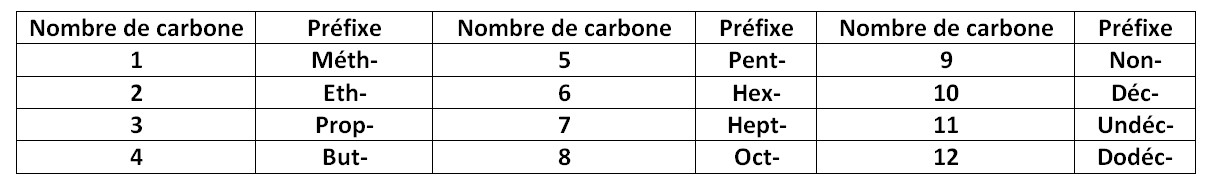
\includegraphics[width=\linewidth]{imgs/c5/prefixe.jpg}
    \caption{Les préfixes IUPAC pour nommer une chaîne en fonction de sa longueur en carbones}
    \label{fig:prefixes}
\end{figure}

\subsubsection{Alcanes}
Les chaîne carbonées ne contenant que des liaisons simples entre les carbones, s'appellent des \textbf{alcanes}\eng{alkane}. Les alcanes sont des hydrocarbures saturés : ils ne contiennent que des atomes de carbone et d’hydrogène liés par des liaisons simples.  Leur formule générale est : $\ce{C_nH_{2n+2}}$.

% Please add the following required packages to your document preamble:
% 
% If you use beamer only pass "xcolor=table" option, i.e. \documentclass[xcolor=table]{beamer}
\begin{table}[H]
\centering
\begin{tabular}{|>{\centering}m{1cm}|c|c|c|c|}
\hline
\rowcolor[HTML]{343434} 
{\color[HTML]{EFEFEF} \tiny{Nombre de Carbone}} & {\color[HTML]{EFEFEF} Nom } & {\color[HTML]{EFEFEF}Formule Brute } & {\color[HTML]{EFEFEF} Formule semi-développée } & {\color[HTML]{EFEFEF}Formule topologique }  \\\hline
1 & Méthane &  &  &  \\[7ex] 
\hline
2 & Ethane &  &  &   \\[7ex] 
\hline
3 & Propane &  &  &   \\[7ex] \hline
4 & Butane &  &  &   \\[7ex] \hline
5& Pentane &  &  &   \\[7ex] \hline
6& Hexane &  &  &   \\[7ex] \hline
7& Heptane &  &  &   \\[7ex] \hline
8& Octane &  &  &   \\[7ex] \hline
9& Nonane &  &  &   \\ [7ex]\hline
10& Décane  &  &  &   \\ [7ex]\hline
11& Undécane &  &  &   \\ [7ex]\hline
12  & Dodécane &  &  &   \\[7ex] \hline
\end{tabular}
\end{table}

\subsubsection{Alcènes}

Les alcènes\eng{alkene} sont des hydrocarbures non-saturés : ils ne contiennent que des atomes de carbone et d’hydrogène liés par des liaisons simples et une liaison double entre deux carbones ($\ce{C=C}$) de la chaîne principale.   Leur formule générale est $\ce{C_nH_{2n}}$  (quand ils comportent une seule liaison double).
	
La nomenclature des alcènes est un peu plus complexe (par rapport aux alcanes), car il faut préciser le placement de la liaison double sur la chaîne principale. Il faut donc utiliser le même nom que celui de l'alcane portant le même nombre d'atomes de carbone, en utilisant la terminaison « -ène » à la place de « -ane », et en intercalant l'indice de position de la double liaison (afin de situer la double liaison, numéroter la chaîne principale de façon à ce que le numéro de l'atome C portant la double liaison soit le plus petit possible) dans le mot, avant le suffixe, et encadré par deux tirets. 

\begin{eg}
\begin{itemize}
    \item $\ce{CH2=CH2}$ s'appelle ethène.
    \item $\ce{CH2=CH-CH2-CH2-CH3}$ s'appelle Pent-1-ène.
    \item \chemfig{
               H_3C% 1
      -[:30,,2]\mcfabove{C}{\mcfright{H}{_2}}% 2
        -[:330]\mcfbelow{C}{H}% 3
         =[:30]\mcfabove{C}{H}% 4
    -[:330,,,1]CH_3% 5
} s'appelle Pent-2-ène.
    \item \chemfig{
               CH_3% 1
     -[:150,,1]\mcfabove{C}{\mcfright{H}{_2}}% 2
        -[:210]\mcfbelow{C}{H}% 3
        =[:150]\mcfabove{C}{H}% 4
    -[:210,,,2]H_3C% 5
} s'appelle Pent-2-ène (car on cherche à numéroter dans le sens qui nous permettrait de minimiser numéro du carbone avec la liaison double).
    \item \chemfig{H-C(-[2]H)(-[6]H)-C(-[2]H)(-[6]H)-C(-[2]H)=C(-[2]H)-C(-[2]H)(-[6]H)-H} est donc la formule développée de Pent-2-ène, avec une formule topologique \chemfig{
           % 1
     -[:30]% 2
    -[:330]% 3
     =[:30]% 4
    -[:330]% 5
}.
\end{itemize}
\end{eg}

\subsubsection{Alcynes}
Il existe une troisième famille d’hydrocarbures, les alcynes\eng{alkyne}, qui sont des chaînes carbonées comportant au moins une liaison triple entre deux carbones ( $\ce{C#C}$ ). Les règles de nomenclature sont comme celles des alcènes sauf pour la terminaison qui devient –yne (comme éthyne, butyne, etc.).  La formule générale d’un alcyne comportant une seule liaison triple est $\ce{C_nH_{2n-2}}$. (Les alcynes ne sont pas au programme de terminale pour le moment). 
\vspace{1.5cm}
\begin{figure}[H]
    \centering
    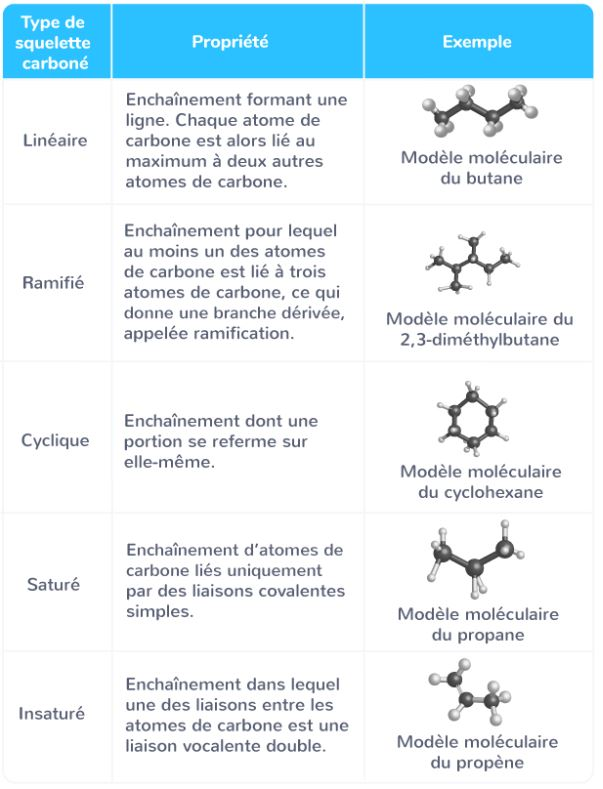
\includegraphics[width=0.75\linewidth]{imgs/c5/structures.jpg}
\end{figure}

\subsubsection{Molécules cycliques}
Lorsque la chaîne est fermée (même partiellement), l’alcane ou l’alcène est dit «cyclique», et le nom est précédé du préfixe cyclo-. 

\begin{eg}

\textbf{Cyclohexane : } en semi-développée
\chemfig{
               \mcfabove{C}{\mcfright{H}{_2}}% 1
        -[:180]\mcfabove{C}{\mcfright{H}{_2}}% 2
    -[:240,,,2]H_2C% 3
     -[:300,,2]\mcfbelow{C}{\mcfright{H}{_2}}% 4
              -\mcfbelow{C}{\mcfright{H}{_2}}% 5
     -[:60,,,1]CH_2% 6
                  (
         -[:120,,1]\phantom{C}% -> 1
                  )
}\quad \quad en topologique
\chemfig{
           % 1
    -[:180]% 2
    -[:240]% 3
    -[:300]% 4
          -% 5
     -[:60]% 6
              (
        -[:120]% -> 1
              )
}
\vspace{1cm}

\textbf{Cyclopentène : } en semi-développéeen
\chemfig{\mcfabove{C}{\mcfright{H}{_2}}-[:180]\mcfabove{C}{\mcfright{H}{_2}}-[:252,,,2]HC=^[:324,,2]\mcfbelow{C}{H}-[:36,,,1]CH_2(-[:108,,1]\phantom{C})} \quad \quad en topologique
\chemfig{
            % 1
     -[:180]% 2
     -[:252]% 3
    =^[:324]% 4
      -[:36]% 5
               (
         -[:108]% -> 1
               )
}


\end{eg}

\begin{rmrq}
\small{Chaque carbone dans une liaison triple doit perdre deux hydrogènes. En commençant donc avec la formule d’un hydrocarbure saturé $(\ce{C_nH_{2n+2}})$ chaque fois que l’on rajoute une liaison entre deux carbones, il faut enlever deux hydrogènes. Ceci est également le cas quand on convertit une chaîne ouverte en chaîne cyclique. Donc en regardant la formule brute d’un hydrocarbure nous pouvons déterminer le nombre de liaisons doubles/triples ou cycliques. }
\end{rmrq}

\begin{rmrq}
\small{Il existe une molécule cyclique particulière, le benzène, $\ce{C6H6}$ composé de 6 carbones cycliques reliés par des liaisons doubles conjuguées. Des molécules contenant un groupe benzène s'appellent souvent des molécules \textit{aromatique}. Le benzène est un précurseur important de nombreux composés organiques, tel que les matières plastiques, des parfums, des additifs alimentaires, et des médicaments. 

\chemfig{\mcfabove{C}{H}=^[:180]\mcfabove{C}{H}-[:240,,,2]HC=^[:300,,2]\mcfbelow{C}{H}-\mcfbelow{C}{H}=^[:60,,,1]CH(-[:120,,1]\phantom{C})}
\quad \quad \quad \chemfig{=^[:180]-[:240]=^[:300]-=^[:60](-[:120])} }
\end{rmrq}

\subsubsection{Ramifications}

Une ramification (ou chaîne latérale) est une chaîne carbonée rattachée à la chaîne principale d’une molécule organique. On les désigne souvent sous le terme générique $\ce{-R}$ ou $\ce{-R'} / \ce{-R''}$ s'il y en a plusieurs. Pour nommer un alcane/ène/yne, le nom de la chaîne principale doit donc être \textbf{précédé} par le nom de la chaîne ramifiée qui est précédé par le numéro du carbone qui la porte. Dans le cas de deux ou plusieurs ramifications, on doit donner l’indice le plus bas au radical prioritaire par ordre alphabétique. 


\begin{figure}[h]
    \centering
    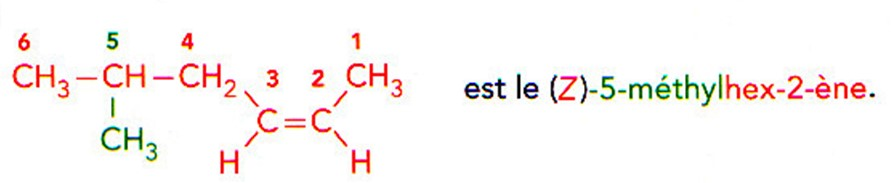
\includegraphics[width=0.65\linewidth]{imgs/c5/ex2.jpg}
\end{figure}

%%%%%%%%%%%%%% ----------------------------------------------------------
\subsection{Groupes caractéristiques \& nomenclature}

\subsubsection*{Alcools}
Un alcool est une molécule organiques comportant un groupe hydroxyle $\ce{-OH}$ sur le squelette carboné. On nomme un alcool en rajoutant une \textbf{terminaison « -ol », précédée par le nombre du carbone fonctionnel}. 

\begin{eg}

\textbf{Ethanol : } 
\chemfig{H_3C-[:330,,2]\mcfbelow{C}{\mcfright{H}{_2}}-[:30,,,1]OH} \quad \quad et en représentation topologique \quad  \chemfig{-[:330]-[:30,,,1]OH}
\vspace{0.5cm}

\textbf{Butan-2-ol : } \chemfig{H_3C-[:330,,2]\mcfbelow{C}{\mcfright{H}{_2}}-[:30]\mcfbelow{C}{H}(-[:90,,,1]OH)-[:330,,,1]CH_3} \quad  et en représentaiton topologique \quad  \chemfig{-[:330]-[:30](-[:90,,,1]OH)-[:330]}
\vspace{.5cm}

\textbf{4-méthylpentan-2-ol : }
\chemfig{CH_3-[:150,,1]\mcfbelow{C}{H}(-[:90,,,1]CH_3)-[:210]\mcfbelow{C}{\mcfright{H}{_2}}-[:150]\mcfbelow{C}{H}(-[:210,,,2]H_3C)-[:90,,,1]OH} et topologique \chemfig{-[:150](-[:90])-[:210]-[:150](-[:90,,,1]OH)-[:210]}
\vspace{.5cm}

\textbf{ 2-méthylpent-2-ène-4-ol : }
\chemfig{CH_2=[:150,,1]C(-[:90,,,1]CH_3)-[:210]\mcfbelow{C}{\mcfright{H}{_2}}-[:150]\mcfbelow{C}{H}(-[:210,,,2]H_3C)-[:90,,,1]OH}  \; et topologique \; \chemfig{=[:150](-[:90])-[:210]-[:150](-[:90,,,1]OH)-[:210]}
\end{eg}

\subsubsection*{Cétones}
Une cétone est une molécule organiques comportant un groupe carbonyle $\ce{C=O}$ sur le squelette carboné. La particularité d'une cétone, par rapport aux autres composés carbonylés, est le fait que le carbone fonctionnel est lié à deux autres carbones. 

On nomme une cétone en rajoutant une terminaison « -one », précédée par le nombre du carbone fonctionnel. 

\begin{eg}

\textbf{Propanone (acétone) : }
\chemfig{H_3C-[:30,,2]C(=[:90]O)-[:330,,,1]CH_3} \quad et en topologique

\textbf{Pentan-2-one : } \hspace{5cm} \textbf{2-méthylhexan-4-one : }
\vspace{2cm}
\end{eg}

\subsubsection*{Esters}
Un ester est une molécule organiques comportant un groupe carbonyle $\ce{C=O}$ associé à un oxygène : $\ce{-CO-O-C-}$. Les esters sont formés dans la réaction entre un alcool et un acide carboxylique (une estérification). De manière générale : $acide\; carboxylique+alcool\rightarrow ester+eau$ ($a+a\rightarrow e+e$) : 
\[ \ce{R1-COOH + R2-OH -> R1-CO-O-R2 + H2O}  \]
\begin{figure}[h]
    \centering
    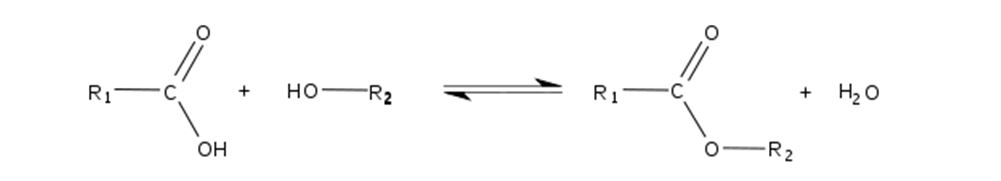
\includegraphics[width=\linewidth]{imgs/c5/esterific.jpg}
\end{figure}

Le nom d'un ester comporte deux termes (un pour l'acide d'origine, et l'autre pour l'alcool d'origine) :
\begin{itemize}
    \item Le premier, avec la terminaison –oate désigne la chaîne carbonée $\ce{R_1-COO-}$ numérotée à partir du carbone fonctionnel ;
    \item Le second, avec la terminaison –yle, est le nom du groupe alkyle $\ce{R_2}$  numéroté à partir de l’atome de carbone lié à l’atome d’oxygène $\ce{O}$. 
\end{itemize}
La \textbf{réaction inverse} d'estérification s'appelle l'\textbf{hydrolyse}. 

\begin{eg}
\begin{itemize}
    \item Ethanol + acide éthanoïque
\vspace{1cm}
	\item butan-2-ol+acide propanoïque
\vspace{1cm}
    \item 3-méthylbutanoate de propyle
\vspace{1cm}
\end{itemize}
\end{eg}

\subsubsection*{Acides carboxyliques}
Un acide carboxylique est une molécule organiques comportant un groupe carboxyle $\ce{-COOH}$ sur le squelette carboné. On nomme un acide carboxylique en rajoutant une terminaison « -oïque », précédée par acide. 

\begin{eg}

\textbf{Acide Propanoïque : } \chemfig{H_3C-[:330,,2]\mcfbelow{C}{\mcfright{H}{_2}}-[:30]C(-[:90,,,1]OH)=[:330]O} \quad \quad \quad \quad \chemfig{-[:330]-[:30](=[:330]O)-[:90,,,1]OH}

\end{eg}

\subsubsection*{Aldéhydes}
Les aldéhydes sont des composés organiques faisant partie de la famille des composés carbonylés, possédant une formule générale : 

Les aldéhydes sont donc des composés carbonylés avec un carbone primaire (i.e. carbone relié à seulement un autre atome de carbone), alors que les cétones sont des composés carbonylés avec un carbone secondaire (i.e. carbone lié à exactement deux atomes de carbone voisins). 

Pour nommer un aldéhyde on ajoute le suffixe ``–al'' au nom de la chaîne principale au lieu de ``–ane''. 

\begin{eg}

\textbf{Méthanal} \hspace{3.5cm} \textbf{Butanal} \hspace{3.5cm} \textbf{3-méthylpentanal}
\vspace{3cm}
\end{eg}

\subsubsection*{Amines}
Une amine est un composé organique dérivé de l’ammoniac dont au moins un hydrogène a été remplacé par une chaîne carbonée. On parle d’amine primaire, secondaire ou tertiaire selon que l’on a un, deux ou trois hydrogènes remplacés par des chaînes carbonées.  

Nomenclature : Le nom d’une amine $\ce{R-NH2}$  dérive de celui de l’alcane de la même chaîne carbonée en remplaçant la terminaison ``–ane'' par la terminaison ``–amine'', précédé de l’indice de position le plus petit possible du groupe amine dans la chaîne carbonée principale. Lorsque l’atome d’azote est lié à d’autres groupes alkyle, le nom de l’amine est précédé de la mention N-alkyl.

\begin{figure}[h]
    \centering
    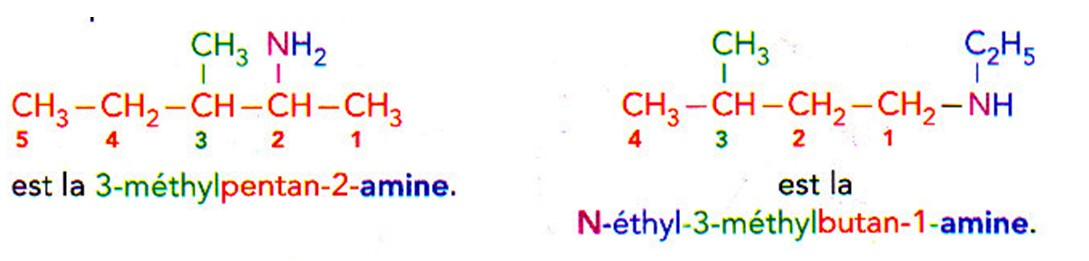
\includegraphics[width=0.85\linewidth]{imgs/c5/exAmine.jpg}
\end{figure}

\subsubsection*{Amides}
Ils sont le produit d’une réaction entre un acide carboxylique et une amine.

Le nom d’un amide dérive de celui de l’alcane de la même chaîne carbonée en remplaçant la terminaison  ``–ane'' par la terminaison ``–amide''. La chaîne carbonée est numérotée à partir du carbone fonctionnel $\ce{C=O}$ . Lorsque l’atome d’azote est lié à des groupes alkyle, le nom de l’amide est précédé de la mention N-alkyl (comme pour les amines).   

\begin{figure}[H]
    \centering
    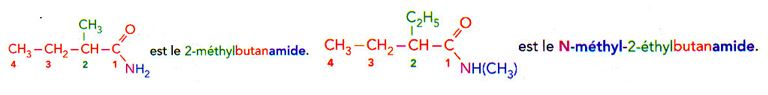
\includegraphics[width=\linewidth]{imgs/c5/exAmide.jpg}
\end{figure}

\begin{figure}[H]
    \centering
    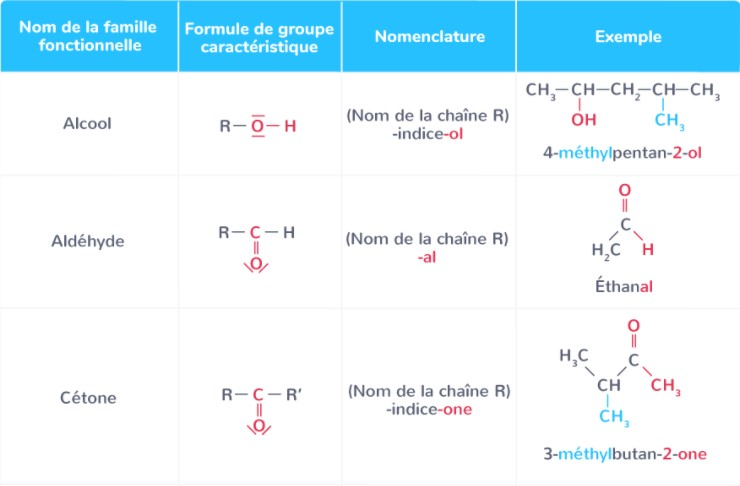
\includegraphics[width=0.85\linewidth]{imgs/c5/groupes1.jpg}
\end{figure}
\begin{figure}[H]
    \centering
    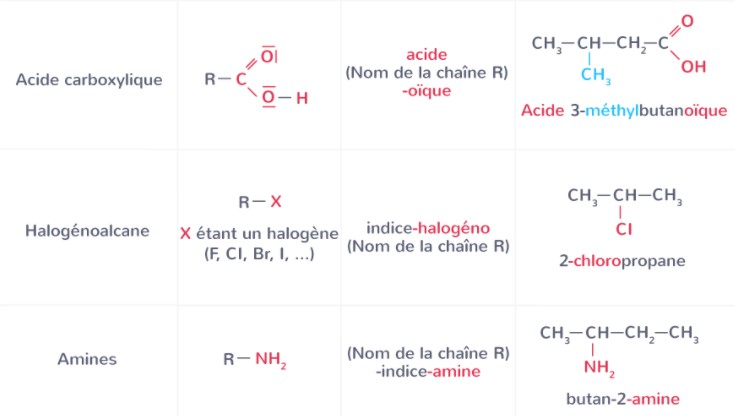
\includegraphics[width=0.85\linewidth]{imgs/c5/groupes2.jpg}
\end{figure}
\begin{figure}[H]
    \centering
    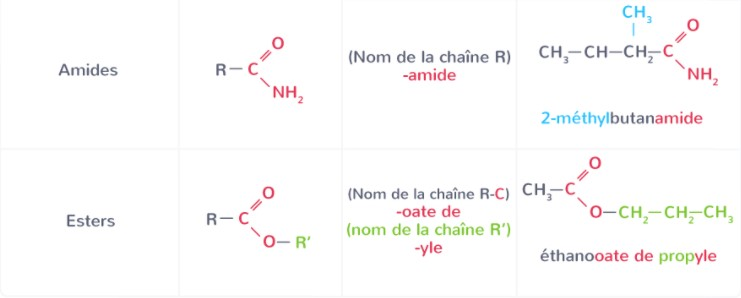
\includegraphics[width=0.85\linewidth]{imgs/c5/groupes3.jpg}
\end{figure}


\subsection{Isomérie}
Vous avez vu la notion d'isomérie pour la première fois en classe de seconde : des molécules ayant la même formule brute (composition) mais ayant des formules développées différentes sont des isomères. Cette définition est correcte, mais insuffisante, car il y a différentes formes d'isomérie. La définition précédente s'appliquent aux \textbf{isomères de constitution}. Mais il y a d'autre formes d'isomères aussi, comme les isomères de configuration, et de conformation : 

\begin{figure}[H]
    \centering
    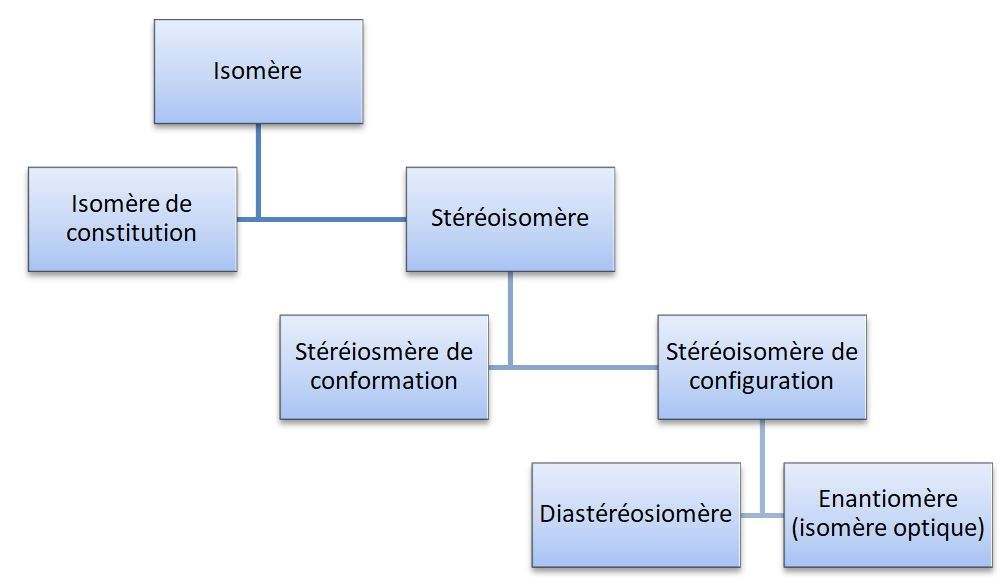
\includegraphics[width=0.85\linewidth]{imgs/c5/isomeres2.jpg}
    \caption{Les différentes types d'isomérie.}
\end{figure}

Nous voyons maintenant, que les isomères rencontrés en secondes sont, en effet, simplement les isomères de constitution. Pour passer d'un isomère de constitution à un autre il est \textbf{obligatoire de briser au moins une liaison} quelque part, sinon les deux molécules sont simplement deux stéréoisomères, et non deux isomères de constitution. Il est important de noter que deux isomères de constitution sont deux molécules différentes, avec des propriétés physico-chimiques différentes (i.e. température de fusion/ébullition, densité, etc...).

\begin{eg} Deux isomères de constitution

Propan-2-ol (gauche) et propan-1-ol/propanol (droite) : 
\chemfig{-[:90](-[:30,,,1]OH)-[:150]}\quad \quad \chemfig{-[:30]-[:330]-[:30,,,1]OH}
\end{eg}

\subsection{Polymères}

Les polymères sont des macromolécules (grandes molécules), composées d'une motif moléculaire (monomère), répété un grand nombre de fois. La plupart des plastiques figurent parmi les polymères (e.g. polystyrène). 

\begin{figure}[ht]
\centering
\begin{subfigure}{.45\textwidth}
  \centering
  % include first image
  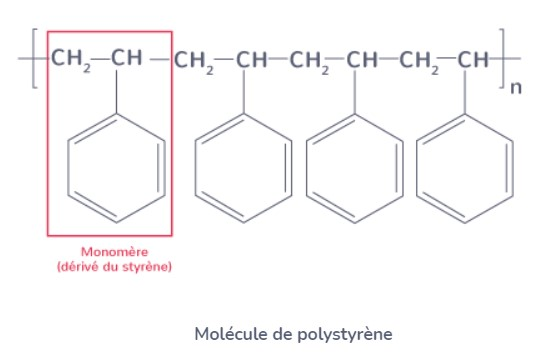
\includegraphics[width=.95\linewidth]{imgs/c5/polymere1.jpg}  
\end{subfigure}
\begin{subfigure}{.45\textwidth}
  \centering
 %%%%%%%%%%% % include first image
  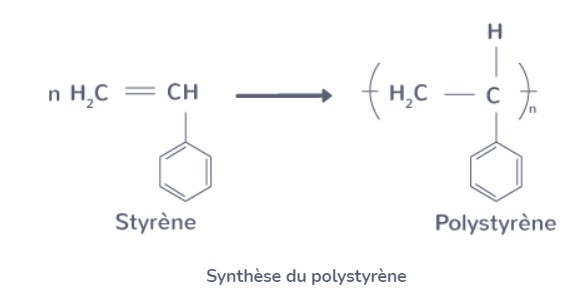
\includegraphics[width=.95\linewidth]{imgs/c5/polymere2.jpg}  
\end{subfigure}
\caption{Le polystyrène et sa synthèse par poly-addition.}
\end{figure}

\section{La synthèse organique}
\begin{defn}{Synthèse}

La synthèse (organique) est la séquence réactionnelle, c'est-à-dire la série des réactions chimiques nécessaires afin de synthétiser une molécule à partir d'une série de réactifs. 
\end{defn}

Pour réaliser une bonne synthèse il faut choisir : 
\begin{itemize}
    \item Les \textbf{réactifs approprié}, ainsi que leurs quantités. souvent l’un des deux est en excès. La réaction est souvent notée par un schéma de synthèse : 
    
    \begin{figure}[h]
    \centering
    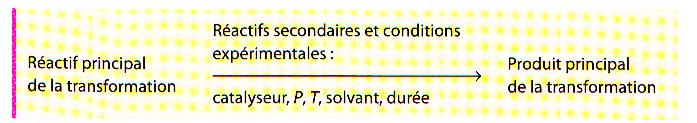
\includegraphics[width=0.95\linewidth]{imgs/c5/syntheseRW.jpg}
\end{figure}

    \item Les \textbf{quantités} (masses ou volumes, masse volumique, etc) des réactifs.
    \item Les \textbf{conditions expérimentales} qui peuvent inclure:
    \begin{itemize}
        \item un \textbf{solvant adapté} qui doit permettre de solubiliser les réactifs. C’est grâce au solvant que les réactifs sont mis en contact. Il n’apparaît pas dans l’équation, mais peut être indiqué dans le schéma de synthèse. 
        \item un \textbf{catalyseur} afin d’accélérer la réaction. Comme pour le solvant on l’indique souvent dans le schéma de la réaction.
        \item les \textbf{paramètres physiques}, comme la température, la pression, etc. \item le \textbf{montage adapté} à la réaction. Par exemple, souvent nous avons besoin de chauffer le mélange réactionnel, pendant une longue période, sans laisser évaporer le contenu. Dans ce cas-là on utilise un montage à reflux, schématiser dans \ref{fig:reflux}. 
    \end{itemize}
\end{itemize}

\begin{figure}[h]
    \centering
    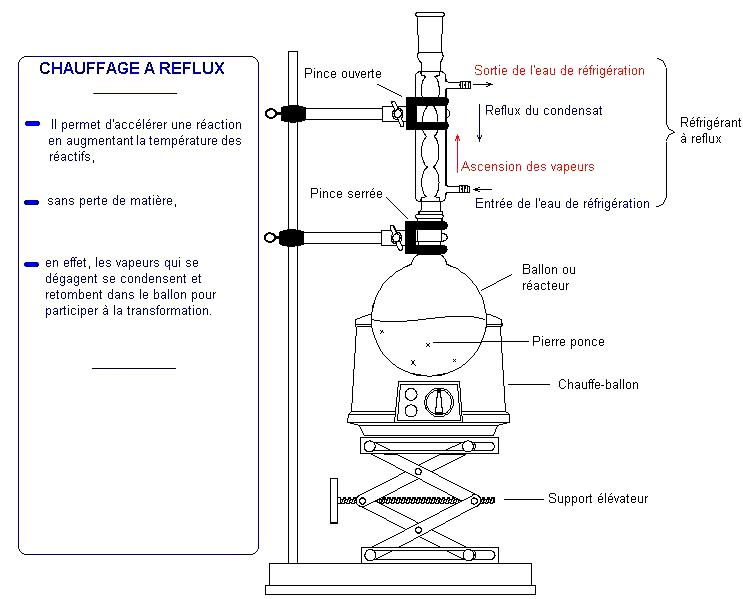
\includegraphics[width=\linewidth]{imgs/c5/reflux2.jpg}
    \caption{Un montage à reflux.}
    \label{fig:reflux}
\end{figure}

Nous allons donc voir, de manière plutôt superficielle, quelles sont les grandes catégories de réaction utiliser dans les synthèses, ainsi que les différentes types de réactions et la modification de la molécule organique qu'elles ciblent. 

\subsection{Différentes types de synthèse}
Tout d'abord nous faisons la distinction entre deux types de réactions: celles visant un modification du squelette carboné, et celles qui visent une modification du ou des groupes caractéristiques. 

\subsubsection{Modification de la chaîne carbonée}

Une grande catégorie des réactions subies par les molécules organiques impliquent une modification de la chaîne carbonée. On peut classifier ces modifications en trois catégories. Des réactions qui entraînent une: 
\begin{itemize}
    \item \textbf{diminution du nombre d’atomes de carbone dans la chaîne}: raccourcissement de la chaîne. 
    \item \textbf{augmentation du nombre d’atomes de carbone dans la chaîne}: allongement de la chaîne.
    \item \textbf{conservation du nombre d’atomes de carbone dans la chaîne}: modification de la structure de la chaîne, sans changer le nombre d'atome de carbone. 
\end{itemize}

Voici quelques exemples de réactions ayant pour but la modification du squelette carbonée de la molécule : 

\textbf{Raccourcissement de la chaîne :} 
Le \textit{craquage catalytique}, utilisé dans l’industrie pétrolière, consiste à casser, à 500°C en présence de catalyseur , les molécules d’hydrocarbures à longue chaîne carbonée en molécules plus petites dont certaines possèdent une double liaison. Exemple : craquage de paraffine en mélange d’alcène. 

\begin{figure}[h]
    \centering
    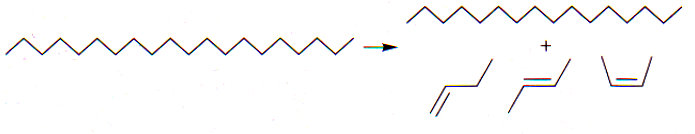
\includegraphics[width=0.8\linewidth]{imgs/c5/craquage.jpg}
\end{figure}

Afin de favoriser la transformation des alcanes en alcènes, le \textit{vapocraquage} est réalisé vers 800°C, en présence de vapeur d’eau.  

\textbf{Allongement de la chaîne : } L'\textit{alkylation} est l’inverse du craquage: il s’agit de la réaction entre petites molécules carbonées pour former une chaîne plus longue. Exemple : 
\begin{figure}[h]
    \centering
    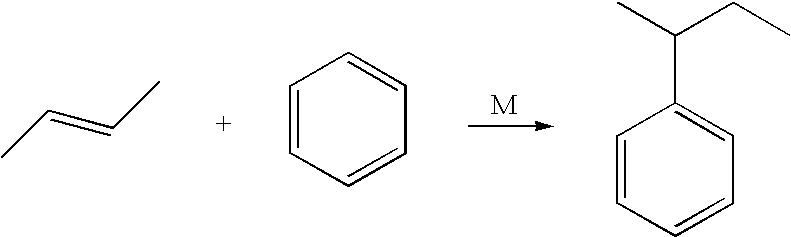
\includegraphics[width=0.8\linewidth]{imgs/c5/alkylation.jpg}
\end{figure}

Un autre exemple, déjà vu, est la \textbf{polymerisation}. 

\textbf{Modification de la structure de la chaîne : }
En général on caractérise une chaîne carbonée en fonction de sa structure qui peut être: \begin{itemize}
    \item linéaire, ramifiée, ou cyclique
    \item saturée (que des liaisons simples)
    \item insaturée (si elle contient au moins une liaison double ou triple)
\end{itemize}
	
Ces modifications font donc varier les paramètres mentionnés ci-avant. Ces modifications sont réalisées, à pression et température élevées en présence de catalyseurs, lors du reformage.

\textit{Isomérisation}: une transformation qui permet de transformer les alcanes linéaires en leurs isomères ramifiés. 
 \begin{figure}[H]
    \centering
    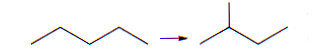
\includegraphics[width=0.65\linewidth]{imgs/c5/isomerisation.jpg}
\end{figure}

\textit{Cyclisation}: une transformation qui permet d’obtenir des cyclanes (alcanes cycliques), souvent ramifiés, et du dihydrogène, à partir des alcanes. Exemple: 

 \begin{figure}[H]
    \centering
    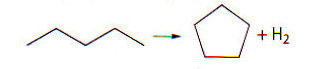
\includegraphics[width=0.65\linewidth]{imgs/c5/cyclisation.jpg}
\end{figure}

\textit{Deshydrogénation}: une transformation qui permet d’obtenir une liaison double dans la chaîne en enlevant une paire d’hydrogène. Exemple: 

\begin{figure}[H]
    \centering
    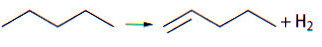
\includegraphics[width=0.65\linewidth]{imgs/c5/deshydrogen.jpg}
\end{figure} 

\textit{Deshydrocyclisation}: une transformation qui permet d’obtenir des dérivés benzéniques et du dihydrogène: 
	
\begin{figure}[H]
    \centering
    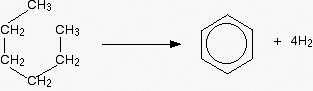
\includegraphics[width=0.7\linewidth]{imgs/c5/deshydrocycle.jpg}
\end{figure}


\subsubsection{Modification du groupe fonctionnel}

On se rappelle que c’est le groupe caractéristique qui confère à une molécule organique la plupart de ses propriétés chimiques importantes. On vise donc une modification de groupe caractéristique lorsqu’on veut une transformation chimique permettant d’ajouter, d’enlever un groupe caractéristique, sans modifier la chaîne principale. 

On ne va pas entrer dans les détails de cette catégorie de modification, mais les réactions d’oxydation et de réduction en font partie.  

Voici quelques exemples: 
\begin{itemize}
    \item Oxydation ménagée de l’octan-2-ol par l’acide hypochloreux $\ce{HClO}$ produit de l’octan-2-one.
    (une réaction générale de forme : $\textsc{ alcool }(groupe\; hydroxyle) \ce{<=>[oxydation][reduction]} \textsc{ cétone }(groupe\; carbonyle)$
    \item Propan-1-ol en présence d’un oxydant en défaut donne du propanal.
    \item Propan-1-ol en présence d’un oxydant en excès donne de l’acide propanoïque.
\end{itemize}

\subsection{Catégories de réaction}
On peut classer la plupart des réactions organiques en trois grandes catégories: 
\begin{itemize}
    \item réactions de \textbf{substitution}
    \item réactions d’\textbf{addition}
    \item réactions d’\textbf{élimination}
\end{itemize}

\subsubsection*{Addition : }
Dans une réaction d’addition, des atomes, ou des groupes d’atomes, sont ajoutés aux atomes d’une liaison multiple. Il existe de nombreuses réactions d’addition (beaucoup trop à mon avis!) En voici quelques exemples: 
\begin{figure}[H]
    \centering
    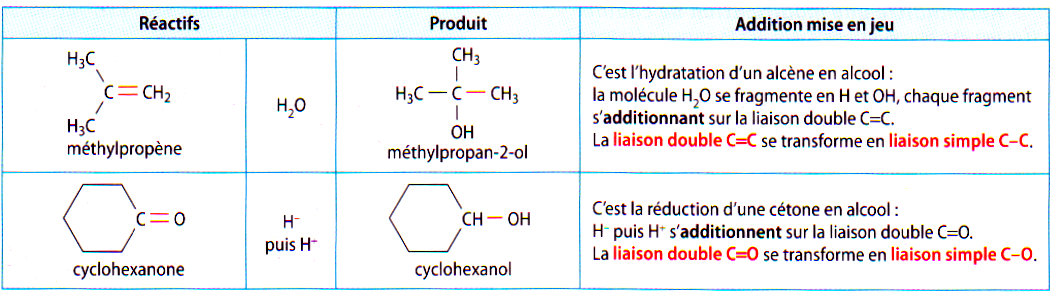
\includegraphics[width=0.8\linewidth]{imgs/c5/addtion.jpg}
\end{figure}
\subsubsection*{Élimination : }
Dans une réaction d’élimination, des atomes ou des groupes d’atomes, protégés par des atomes adjacents, sont éliminés pour former une liaison multiple. 
\begin{figure}[H]
    \centering
    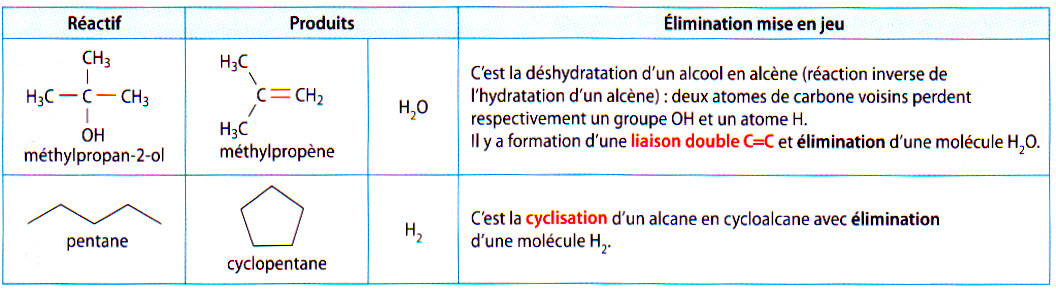
\includegraphics[width=0.8\linewidth]{imgs/c5/elimination.jpg}
\end{figure}
\subsubsection*{Substitution : }
Dans une réaction de substitution, un atome ou un groupe d’atomes est remplacé par un autre atome ou groupe d’atomes. Exemples: 
\begin{figure}[H]
    \centering
    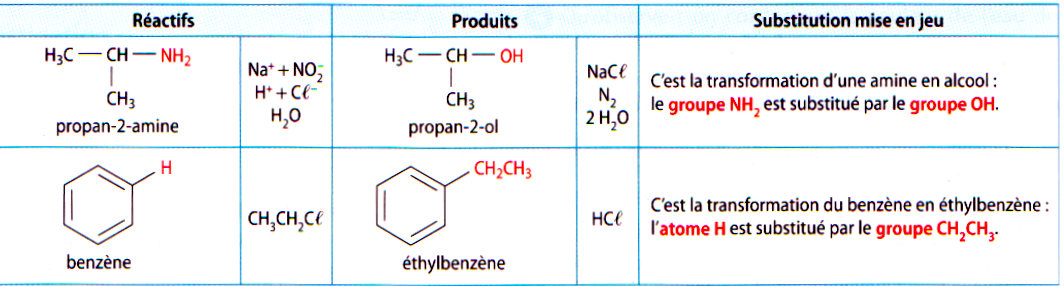
\includegraphics[width=0.8\linewidth]{imgs/c5/substitute.jpg}
\end{figure} 

\section{Stratégies de synthèse}
Étant donné que la synthèse organique est la partie intégrale de la chimie organique, que ce soit dans un domaine de recherche, ou dans un domaine plus industriel (pharmaceutique, pétrolier, etc), les stratégies de synthèse font une partie intégrale de la synthèse, non-seulement dans le but d'optimiser la production, et faire des économies, mais aussi dans un but environnemental. 

\subsection{Optimisation d'une étape}
Ayant déjà abordé les notions concernant la cinétique chimique, nous pouvons voir plus facilement comment il est possible d'optimiser une synthèse organique en jouant sur les facteur cinétiques. 

L'optimisation peut être l'augmentation de la vitesse d'une réaction, mais aussi l'augmentation du rendement d'une réaction, ou encore augmentation de la sélectivité d'une réaction. 

Pour augmenter la vitesse d'une réaction nous avons plusieurs facteur cinétiques à manipuler : 
\begin{itemize}
    \item Concentration des réactifs à l'état initial
    \item Température du milieu de réaction
    \item Addition d'un catalyseur
\end{itemize}
Voici pourquoi un montage à reflux est souvent utilisé dans des synthèses organiques. 

\subsection{Rendement d'une réaction \& son optimisation}

\begin{defn}{Rendement de réaction \eng{chemical yield}}
\begin{itemize}
    \item On appelle rendement $\eta$(éta) d’une réaction le quotient de la quantité du produit effectivement obtenue $n_{exp}$  par la quantité maximale attendue, $n_{th}$.
    \item Le rendement s'exprime : \[ \eta = \frac{n_{exp}}{n_{th}} \]
    \item Le rendement de la synthèse est, dans le cas d’une synthèse multi-étape, égal au produit des rendements de chaque étape 
\end{itemize}
\end{defn}

Le rendement de la réaction (comme la notion de rendement, en physique) est une \textbf{mesure de l'efficacité de la réaction  dans la conversion des réactifs en produit}. Il est donc désirable d'augmenter le rendement d'une réaction donnée, afin de favoriser la formation des produits. Ceci peut se faire par :
\begin{itemize}
    \item L'introduction d'un des réactifs en excès. 
    \item L'élimination d'un des produits, du milieu réactionnel, pendant la synthèse. 
\end{itemize}
En effet - comme j'imagine vous avez déjà compris - dans les deux cas, on \textbf{joue sur le quotient de la réaction} : on le modifie dans le but de faire \textbf{avancer la réaction dans le sens direct}, favorisant la formation des produits. c'est-à-dire \textbf{on force un déplacement de l'équilibre}. 

Dans le premier cas on diminue le quotient en augmentant le dénominateur; et dans le deuxième cas on diminue le numérateur. Dans les deux cas, une fois $Q_r<K$ la réaction avance dans le sens directe, afin de rétablir l'équilibre, et mettre à terme la réaction. 
\newpage
\subsection{Protection \& déprotection}
\begingroup
\begin{wrapfigure}{r}{0.3\textwidth}
\centering
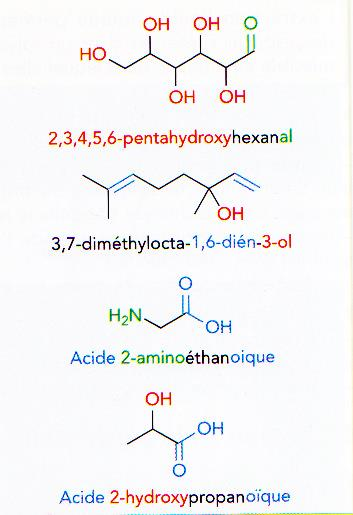
\includegraphics[width=0.3\textwidth]{imgs/c5/polyfonct1.jpg}
%\vspace{-5pt}
\end{wrapfigure}

\begin{defn}{Molécule polyfonctionnelle}

Une molécule polyfonctionnelle est une molécule qui présente plusieurs groupes caractéristiques.

\end{defn}
\vspace{1cm}
\begin{defn}{Réactif chimiosoéléctif}

Une \textbf{réaction est sélective} lorsque, parmi plusieurs fonctions d’une même molécule, l’une d’elles réagit préférentiellement avec le réactif considéré. 

Un \textbf{réactif chimiosélectif} est une espèce chimique qui ne transforme, dans des conditions données, qu’un seul groupe ou type de groupe caractéristique de la molécule polyfonctionnelle avec laquelle il réagit. 
\end{defn}
\vspace{0.5cm}

\endgroup

Il peut être nécessaire que lors d'une réaction, un des groupes caractéristiques doit être protégé, pour éviter qu'il soit modifié par la synthèse. 

Dans cette situation, il y a des étapes supplémentaires rajoutées à la synthèse afin de \textbf{protéger les groupes}. Pour cela nous utilisons un composé qui s'appelle un ``groupe protecteur''. 

\begin{defn}{Groupe protecteur}
\begin{itemize}
    \item Un groupe protecteur est un groupe caractéristique, volontairement créé dans la molécule d’un composé polyfonctionnel afin de \textbf{bloquer la réactivité} de l’une de ses fonctions. Cette fonction est temporairement transformée en une autre fonction. 
    \item Le groupe protecteur utilisé doit :
    \begin{itemize}
        \item Réagir de manière \textbf{sélective} avec la fonction à protéger
        \item Être \textbf{stable} lors des réactions suivantes ;
        \item Pouvoir être \textbf{enlevé (clivé) facilement} et de manière sélective en fin de la réaction. 
    \end{itemize}
    \item La protection d’un groupe ajoute \textbf{au moins deux étapes} à la synthèse. Il faut donc que les étapes de protection et de déprotection aient lieu avec de très bons rendements. 
\end{itemize}
\end{defn}

De manière générale le déroulement se fait en trois étapes : 
\begin{enumerate}
    \item \textbf{Protection : }La réaction a lieu entre le groupe protecteur et le/les groupe(s) caractéristique(s) à protéger. 
    \item \textbf{Réaction de synthèse : }La réaction de la synthèse a lieu, comme prévu. 
    \item \textbf{Déprotection : }La réaction inverse de la première étape a lieu, dans le but d'enlever le groupe protecteur. 
\end{enumerate}

\begin{figure}[ht]
\centering
\begin{subfigure}{.48\textwidth}
  \centering
  % include first image
  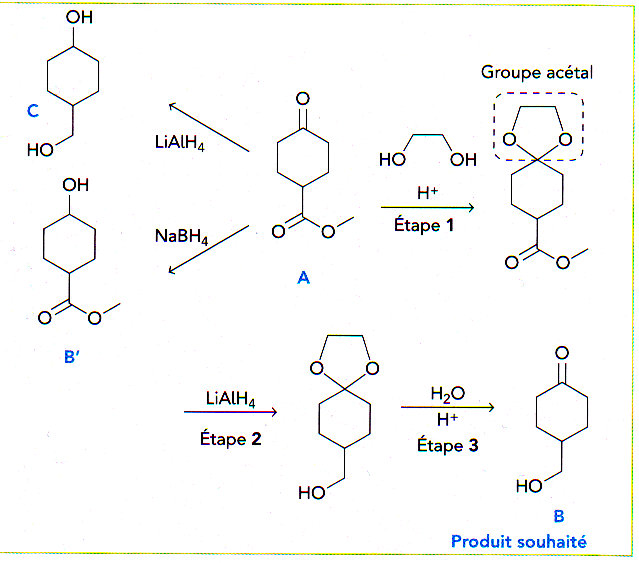
\includegraphics[width=.95\linewidth]{imgs/c5/protect.jpg}  
\end{subfigure}
\begin{subfigure}{.48\textwidth}
  \centering
  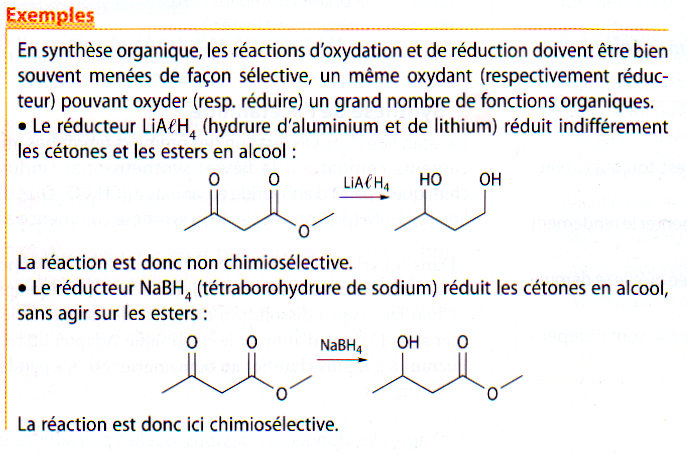
\includegraphics[width=.95\linewidth]{imgs/c5/protect2.jpg}  
\end{subfigure}
\caption{Deux exemples de réactions nécessitant de la protection.}
\end{figure}

\subsection{Synthèse éco-responsable}

Depuis un certain nombre d'année, les facteur matériels et économiques ne sont plus les seuls à considérer dans la conception des synthèses organiques. L'impact environnemental des processus chimiques est un facteur aussi important dans cette conception. 

Douzes principes ont étés proposer à respecter, par les chimistes américains Paul Anastas et John C. Warner en 1998, dont : 

\begin{itemize}
    \item \textbf{Prévention} : il vaut mieux produire moins de déchets qu'investir dans l'assainissement ou l'élimination des déchets.
    \item L'\textbf{économie d'atomes} : les synthèses doivent être conçues dans le but de maximiser l'incorporation des matériaux utilisés au cours du procédé dans le produit final.
    \item Lorsque c'est possible, il faut \textbf{supprimer l'utilisation de substances auxiliaires} (solvants, agents de séparation, ...) ou utiliser des substances inoffensives
    \item Lorsque la technologie et les moyens financiers le permettent, les matières premières utilisées doivent être \textbf{renouvelables} plutôt que non-renouvelables.
\end{itemize}

\begin{figure}[H]
    \centering
    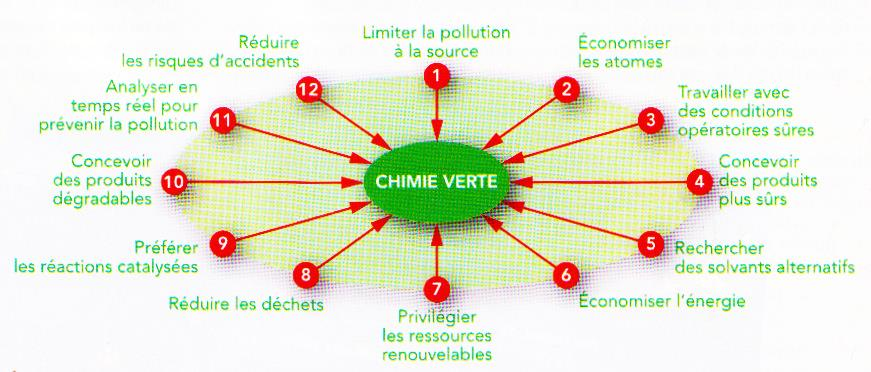
\includegraphics[width=\linewidth]{imgs/c5/12principes.jpg}
\end{figure} 

Un des points les plus importants et les plus centraux est la question de carbone, et l’addition du carbone (sous forme de dioxyde de carbone principalement). C’est le carbone qui joue le rôle centrale dans la crise croissante (et potentiellement existentielle) du changement climatique. Par conséquent, la plus part de la réflexion et de la recherche tournent autour de la question de la maîtrise de notre procuration, utilisation et rejet du carbone dans notre environnement planétaire. Nous allons donc rencontrer des notions comme la \textbf{séquestration} ou la \textbf{valorisation} du carbone. 
\begin{figure}[H]
    \centering
    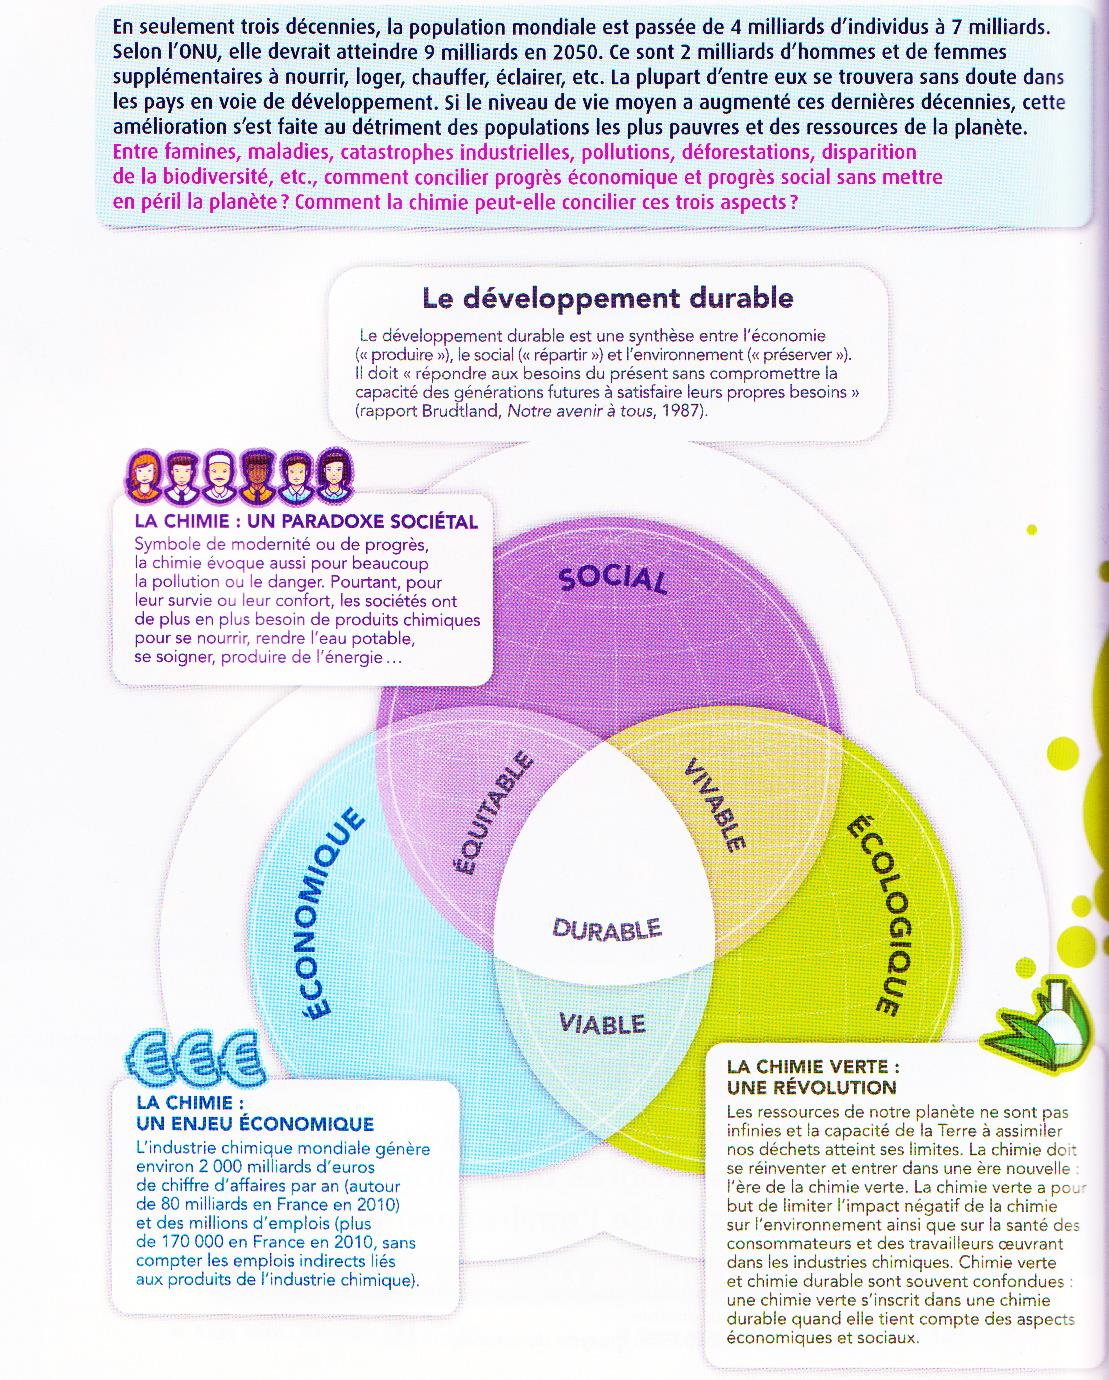
\includegraphics[width=\linewidth]{imgs/c5/vert1.jpg}
\end{figure} 
\begin{figure}[H]
    \centering
    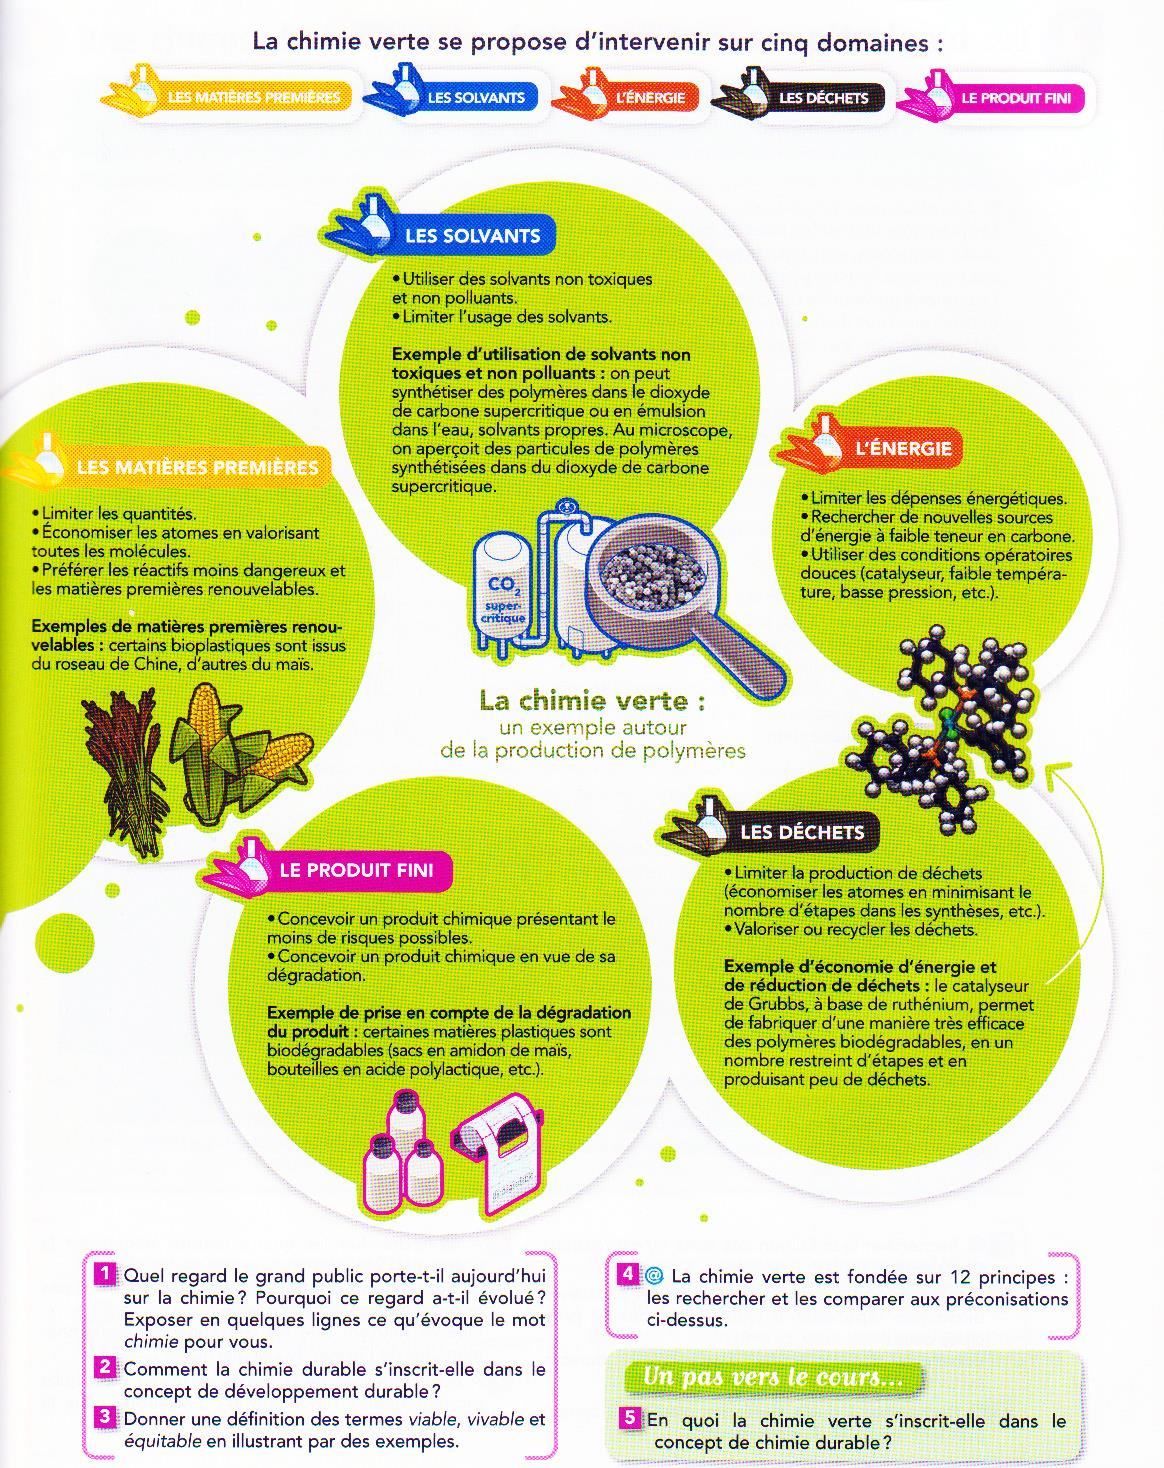
\includegraphics[width=\linewidth]{imgs/c5/vert2.jpg}
\end{figure} 

\section*{Pour résumer ... }

\begin{figure}[H]
    \centering
    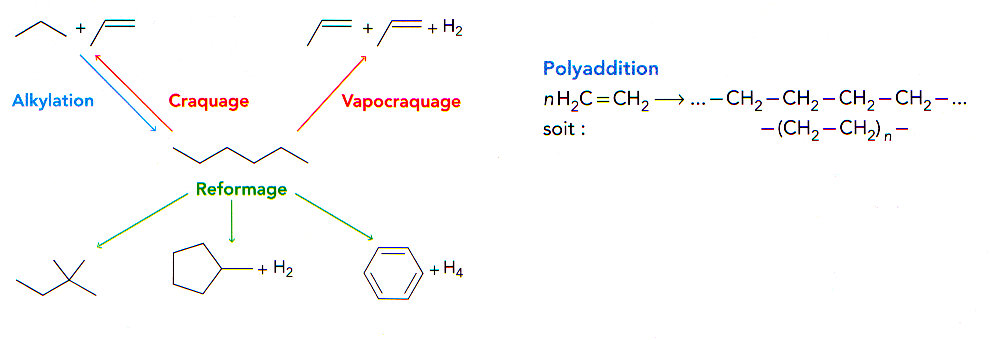
\includegraphics[width=0.95\linewidth]{imgs/c5/synthRECAP.jpg}
\end{figure}

\begin{figure}[H]
    \centering
    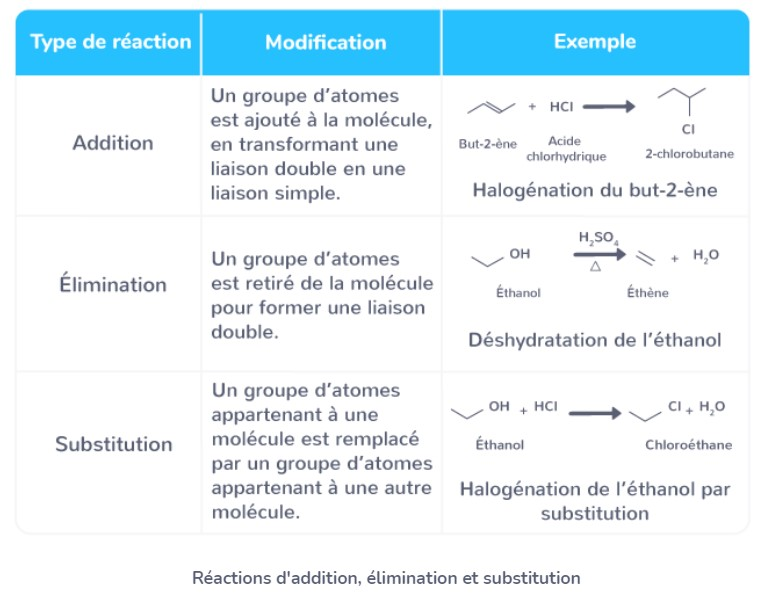
\includegraphics[width=0.95\linewidth]{imgs/c5/catRX.jpg}
\end{figure}

\begin{figure}[H]
    \centering
    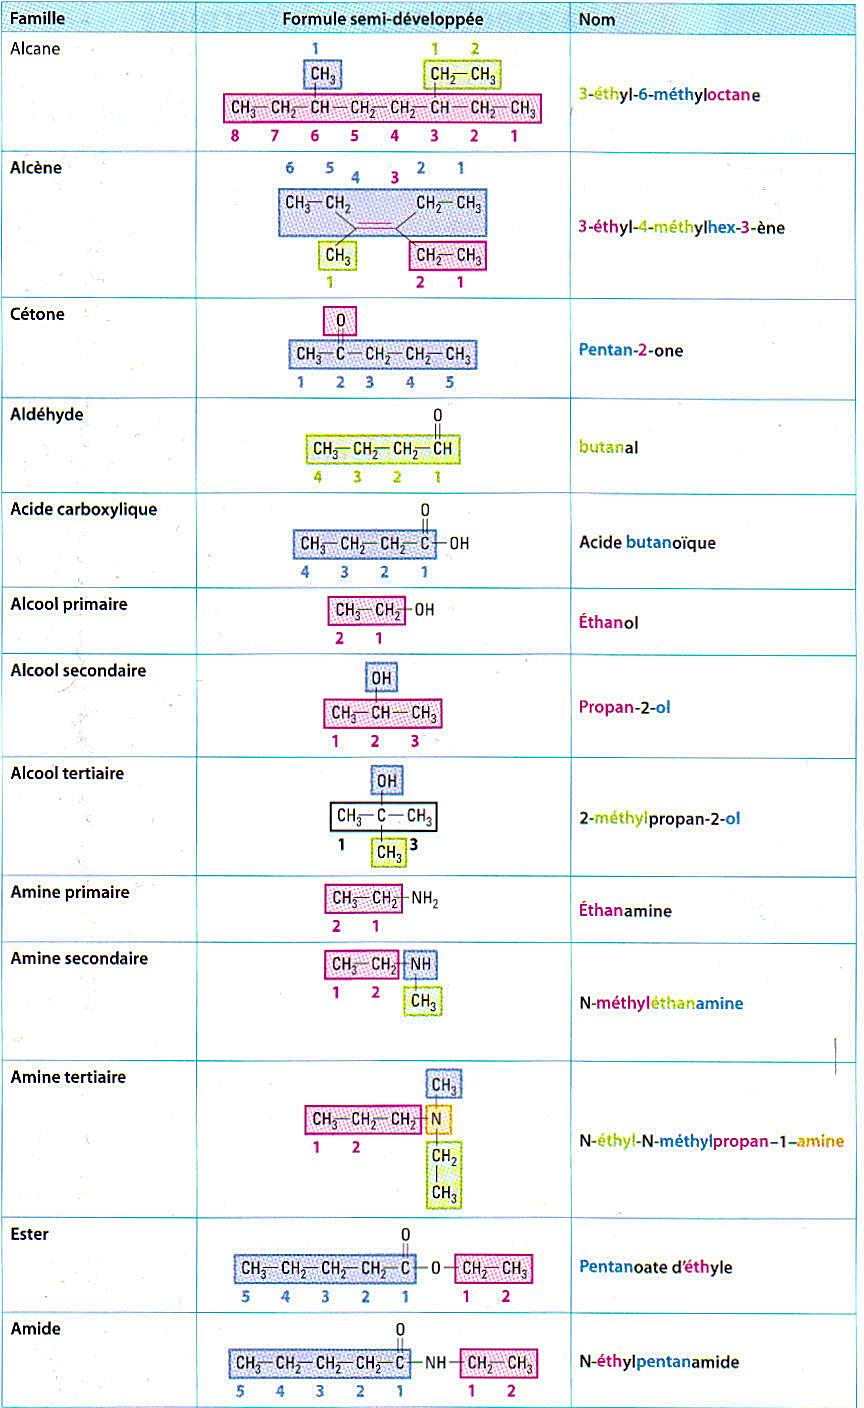
\includegraphics[width=.9\linewidth]{imgs/c5/recapgroupes.jpg}
\end{figure}

\begin{figure}[H]
    \centering
    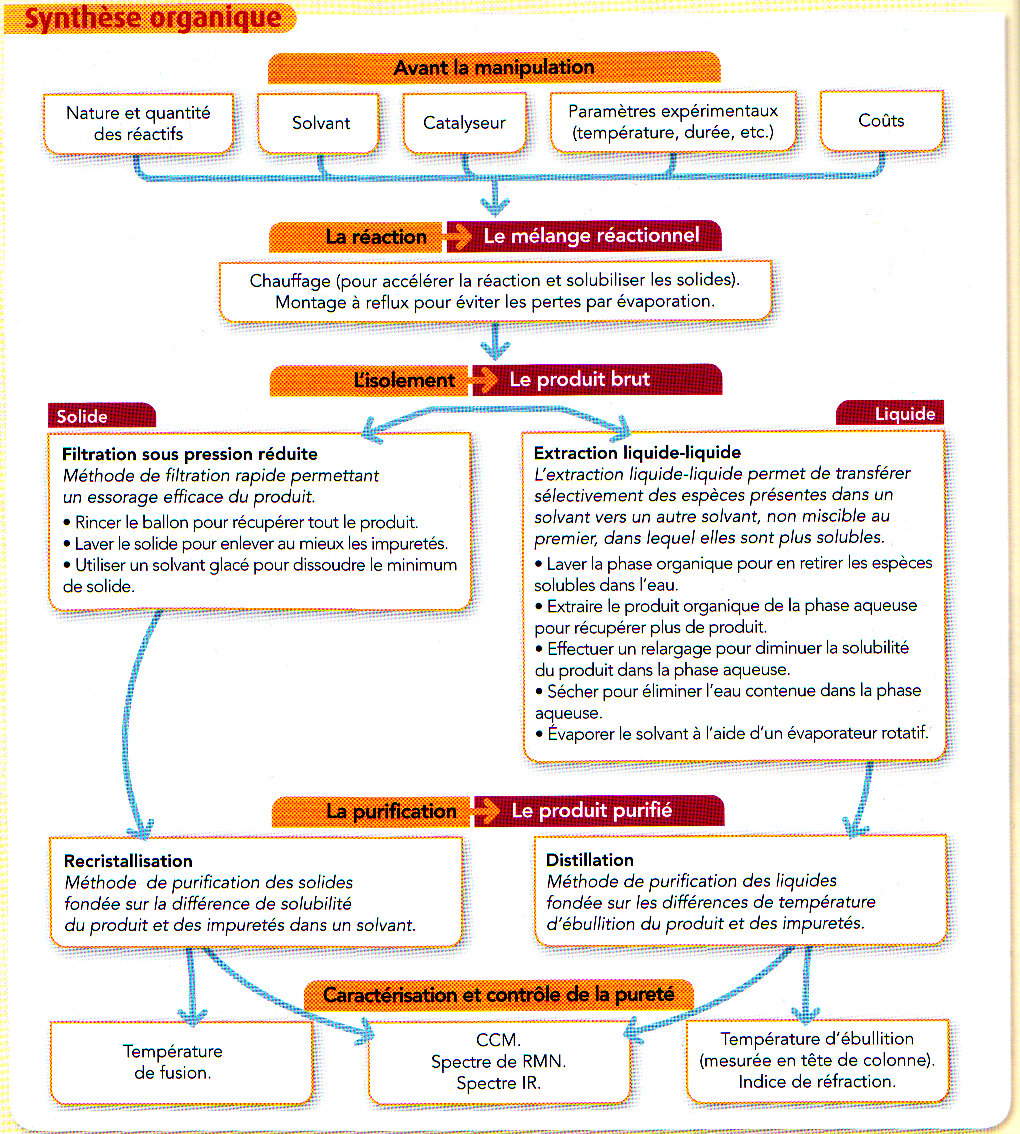
\includegraphics[width=\linewidth]{imgs/c5/recapSynth.jpg}
\end{figure}

\section{Exercices résolus}
\begin{figure}[H]
    \centering
    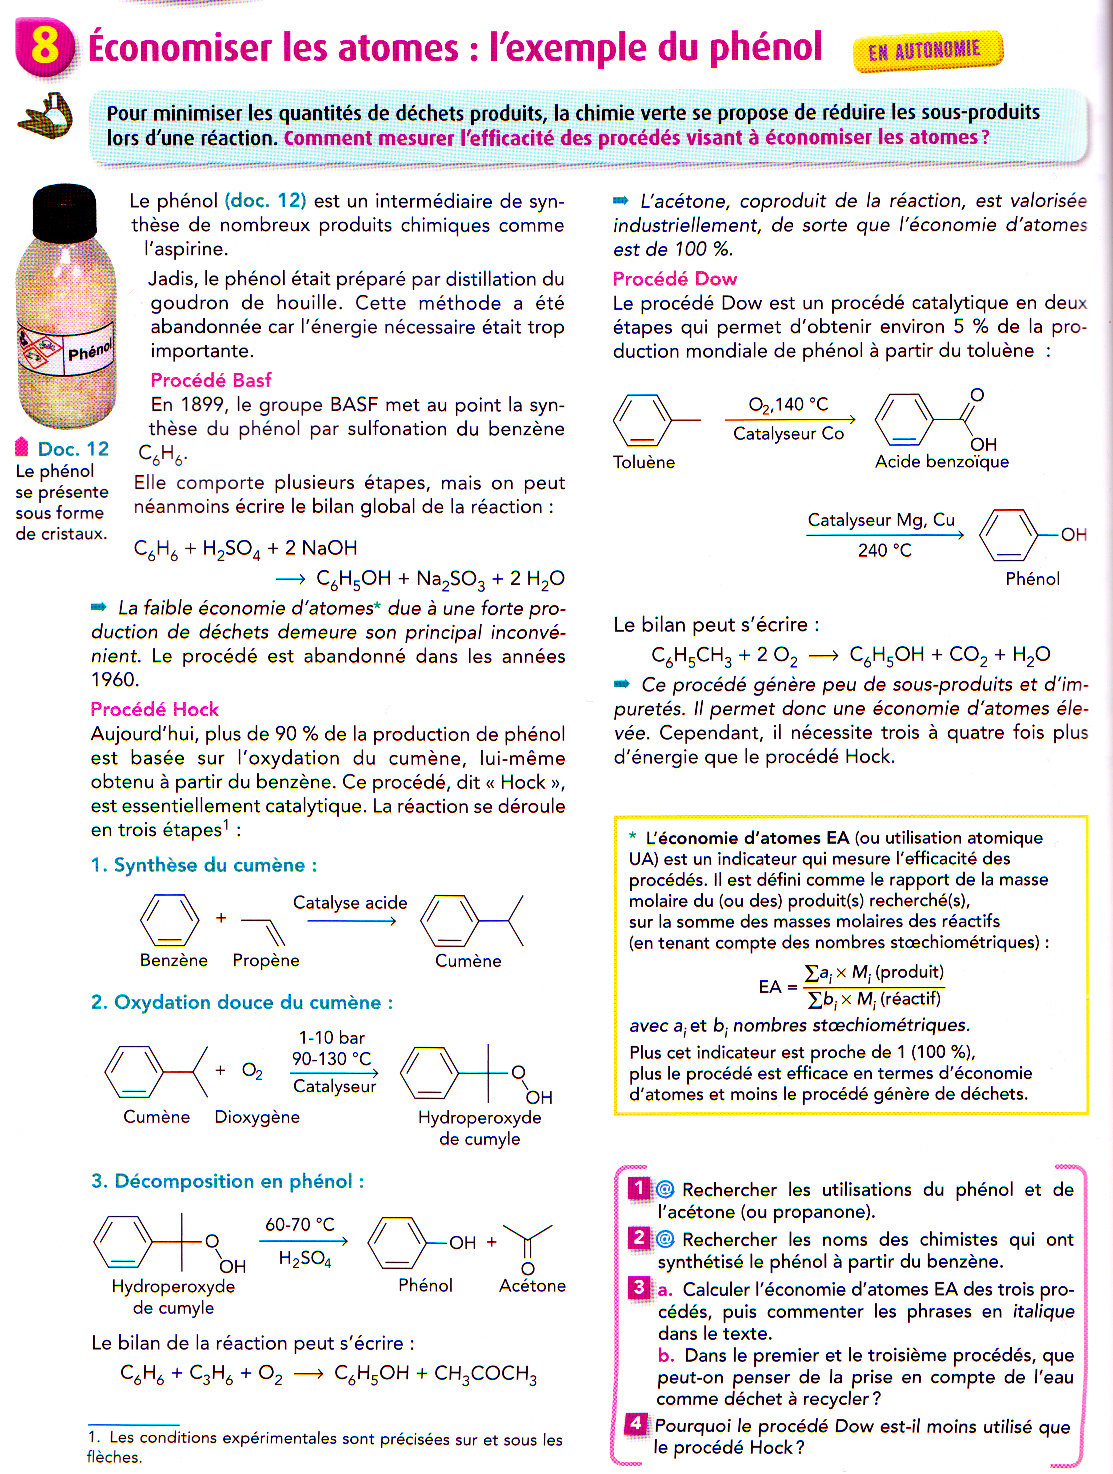
\includegraphics[width=\linewidth]{imgs/c5/xoVert.jpg}
\end{figure}

\begin{figure}[H]
    \centering
    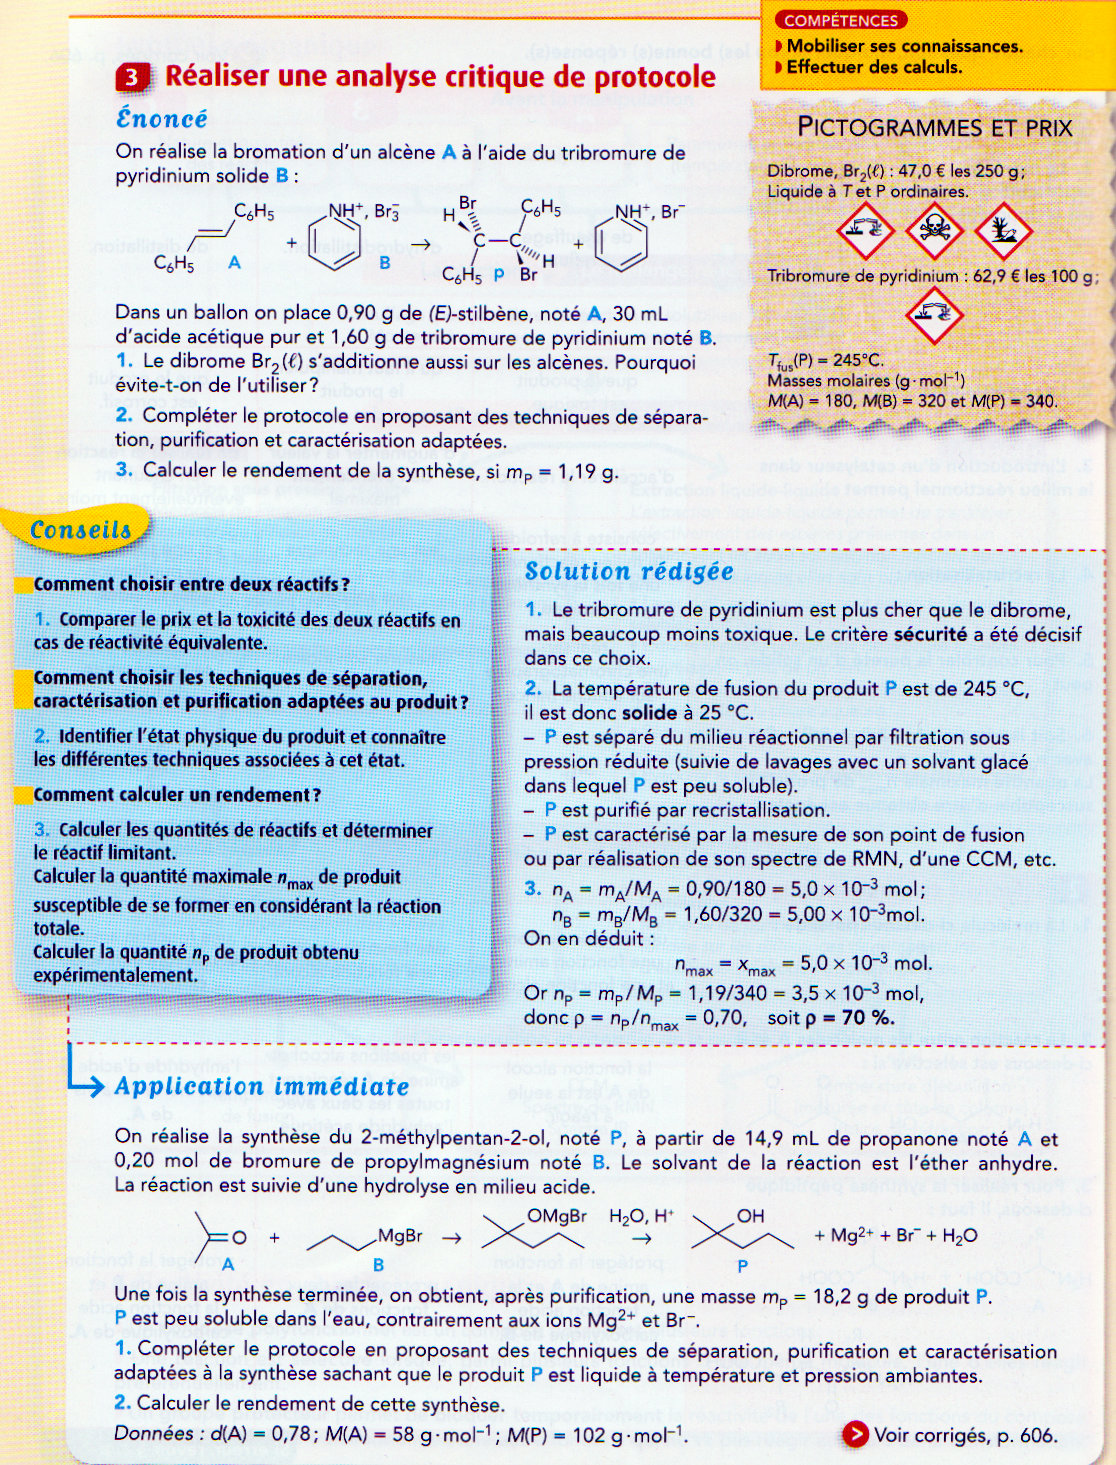
\includegraphics[width=\linewidth]{imgs/c5/xosynth2.jpg}
\end{figure}








\end{document}